% Options for packages loaded elsewhere
\PassOptionsToPackage{unicode}{hyperref}
\PassOptionsToPackage{hyphens}{url}
\PassOptionsToPackage{dvipsnames,svgnames,x11names}{xcolor}
%
\documentclass[
  letterpaper,
  DIV=11,
  numbers=noendperiod]{scrreprt}

\usepackage{amsmath,amssymb}
\usepackage{lmodern}
\usepackage{iftex}
\ifPDFTeX
  \usepackage[T1]{fontenc}
  \usepackage[utf8]{inputenc}
  \usepackage{textcomp} % provide euro and other symbols
\else % if luatex or xetex
  \usepackage{unicode-math}
  \defaultfontfeatures{Scale=MatchLowercase}
  \defaultfontfeatures[\rmfamily]{Ligatures=TeX,Scale=1}
\fi
% Use upquote if available, for straight quotes in verbatim environments
\IfFileExists{upquote.sty}{\usepackage{upquote}}{}
\IfFileExists{microtype.sty}{% use microtype if available
  \usepackage[]{microtype}
  \UseMicrotypeSet[protrusion]{basicmath} % disable protrusion for tt fonts
}{}
\makeatletter
\@ifundefined{KOMAClassName}{% if non-KOMA class
  \IfFileExists{parskip.sty}{%
    \usepackage{parskip}
  }{% else
    \setlength{\parindent}{0pt}
    \setlength{\parskip}{6pt plus 2pt minus 1pt}}
}{% if KOMA class
  \KOMAoptions{parskip=half}}
\makeatother
\usepackage{xcolor}
\setlength{\emergencystretch}{3em} % prevent overfull lines
\setcounter{secnumdepth}{5}
% Make \paragraph and \subparagraph free-standing
\ifx\paragraph\undefined\else
  \let\oldparagraph\paragraph
  \renewcommand{\paragraph}[1]{\oldparagraph{#1}\mbox{}}
\fi
\ifx\subparagraph\undefined\else
  \let\oldsubparagraph\subparagraph
  \renewcommand{\subparagraph}[1]{\oldsubparagraph{#1}\mbox{}}
\fi

\usepackage{color}
\usepackage{fancyvrb}
\newcommand{\VerbBar}{|}
\newcommand{\VERB}{\Verb[commandchars=\\\{\}]}
\DefineVerbatimEnvironment{Highlighting}{Verbatim}{commandchars=\\\{\}}
% Add ',fontsize=\small' for more characters per line
\usepackage{framed}
\definecolor{shadecolor}{RGB}{241,243,245}
\newenvironment{Shaded}{\begin{snugshade}}{\end{snugshade}}
\newcommand{\AlertTok}[1]{\textcolor[rgb]{0.68,0.00,0.00}{#1}}
\newcommand{\AnnotationTok}[1]{\textcolor[rgb]{0.37,0.37,0.37}{#1}}
\newcommand{\AttributeTok}[1]{\textcolor[rgb]{0.40,0.45,0.13}{#1}}
\newcommand{\BaseNTok}[1]{\textcolor[rgb]{0.68,0.00,0.00}{#1}}
\newcommand{\BuiltInTok}[1]{\textcolor[rgb]{0.00,0.23,0.31}{#1}}
\newcommand{\CharTok}[1]{\textcolor[rgb]{0.13,0.47,0.30}{#1}}
\newcommand{\CommentTok}[1]{\textcolor[rgb]{0.37,0.37,0.37}{#1}}
\newcommand{\CommentVarTok}[1]{\textcolor[rgb]{0.37,0.37,0.37}{\textit{#1}}}
\newcommand{\ConstantTok}[1]{\textcolor[rgb]{0.56,0.35,0.01}{#1}}
\newcommand{\ControlFlowTok}[1]{\textcolor[rgb]{0.00,0.23,0.31}{#1}}
\newcommand{\DataTypeTok}[1]{\textcolor[rgb]{0.68,0.00,0.00}{#1}}
\newcommand{\DecValTok}[1]{\textcolor[rgb]{0.68,0.00,0.00}{#1}}
\newcommand{\DocumentationTok}[1]{\textcolor[rgb]{0.37,0.37,0.37}{\textit{#1}}}
\newcommand{\ErrorTok}[1]{\textcolor[rgb]{0.68,0.00,0.00}{#1}}
\newcommand{\ExtensionTok}[1]{\textcolor[rgb]{0.00,0.23,0.31}{#1}}
\newcommand{\FloatTok}[1]{\textcolor[rgb]{0.68,0.00,0.00}{#1}}
\newcommand{\FunctionTok}[1]{\textcolor[rgb]{0.28,0.35,0.67}{#1}}
\newcommand{\ImportTok}[1]{\textcolor[rgb]{0.00,0.46,0.62}{#1}}
\newcommand{\InformationTok}[1]{\textcolor[rgb]{0.37,0.37,0.37}{#1}}
\newcommand{\KeywordTok}[1]{\textcolor[rgb]{0.00,0.23,0.31}{#1}}
\newcommand{\NormalTok}[1]{\textcolor[rgb]{0.00,0.23,0.31}{#1}}
\newcommand{\OperatorTok}[1]{\textcolor[rgb]{0.37,0.37,0.37}{#1}}
\newcommand{\OtherTok}[1]{\textcolor[rgb]{0.00,0.23,0.31}{#1}}
\newcommand{\PreprocessorTok}[1]{\textcolor[rgb]{0.68,0.00,0.00}{#1}}
\newcommand{\RegionMarkerTok}[1]{\textcolor[rgb]{0.00,0.23,0.31}{#1}}
\newcommand{\SpecialCharTok}[1]{\textcolor[rgb]{0.37,0.37,0.37}{#1}}
\newcommand{\SpecialStringTok}[1]{\textcolor[rgb]{0.13,0.47,0.30}{#1}}
\newcommand{\StringTok}[1]{\textcolor[rgb]{0.13,0.47,0.30}{#1}}
\newcommand{\VariableTok}[1]{\textcolor[rgb]{0.07,0.07,0.07}{#1}}
\newcommand{\VerbatimStringTok}[1]{\textcolor[rgb]{0.13,0.47,0.30}{#1}}
\newcommand{\WarningTok}[1]{\textcolor[rgb]{0.37,0.37,0.37}{\textit{#1}}}

\providecommand{\tightlist}{%
  \setlength{\itemsep}{0pt}\setlength{\parskip}{0pt}}\usepackage{longtable,booktabs,array}
\usepackage{calc} % for calculating minipage widths
% Correct order of tables after \paragraph or \subparagraph
\usepackage{etoolbox}
\makeatletter
\patchcmd\longtable{\par}{\if@noskipsec\mbox{}\fi\par}{}{}
\makeatother
% Allow footnotes in longtable head/foot
\IfFileExists{footnotehyper.sty}{\usepackage{footnotehyper}}{\usepackage{footnote}}
\makesavenoteenv{longtable}
\usepackage{graphicx}
\makeatletter
\def\maxwidth{\ifdim\Gin@nat@width>\linewidth\linewidth\else\Gin@nat@width\fi}
\def\maxheight{\ifdim\Gin@nat@height>\textheight\textheight\else\Gin@nat@height\fi}
\makeatother
% Scale images if necessary, so that they will not overflow the page
% margins by default, and it is still possible to overwrite the defaults
% using explicit options in \includegraphics[width, height, ...]{}
\setkeys{Gin}{width=\maxwidth,height=\maxheight,keepaspectratio}
% Set default figure placement to htbp
\makeatletter
\def\fps@figure{htbp}
\makeatother

\KOMAoption{captions}{tableheading}
\makeatletter
\@ifpackageloaded{tcolorbox}{}{\usepackage[many]{tcolorbox}}
\@ifpackageloaded{fontawesome5}{}{\usepackage{fontawesome5}}
\definecolor{quarto-callout-color}{HTML}{909090}
\definecolor{quarto-callout-note-color}{HTML}{0758E5}
\definecolor{quarto-callout-important-color}{HTML}{CC1914}
\definecolor{quarto-callout-warning-color}{HTML}{EB9113}
\definecolor{quarto-callout-tip-color}{HTML}{00A047}
\definecolor{quarto-callout-caution-color}{HTML}{FC5300}
\definecolor{quarto-callout-color-frame}{HTML}{acacac}
\definecolor{quarto-callout-note-color-frame}{HTML}{4582ec}
\definecolor{quarto-callout-important-color-frame}{HTML}{d9534f}
\definecolor{quarto-callout-warning-color-frame}{HTML}{f0ad4e}
\definecolor{quarto-callout-tip-color-frame}{HTML}{02b875}
\definecolor{quarto-callout-caution-color-frame}{HTML}{fd7e14}
\makeatother
\makeatletter
\makeatother
\makeatletter
\@ifpackageloaded{bookmark}{}{\usepackage{bookmark}}
\makeatother
\makeatletter
\@ifpackageloaded{caption}{}{\usepackage{caption}}
\AtBeginDocument{%
\ifdefined\contentsname
  \renewcommand*\contentsname{Table of contents}
\else
  \newcommand\contentsname{Table of contents}
\fi
\ifdefined\listfigurename
  \renewcommand*\listfigurename{List of Figures}
\else
  \newcommand\listfigurename{List of Figures}
\fi
\ifdefined\listtablename
  \renewcommand*\listtablename{List of Tables}
\else
  \newcommand\listtablename{List of Tables}
\fi
\ifdefined\figurename
  \renewcommand*\figurename{Figure}
\else
  \newcommand\figurename{Figure}
\fi
\ifdefined\tablename
  \renewcommand*\tablename{Table}
\else
  \newcommand\tablename{Table}
\fi
}
\@ifpackageloaded{float}{}{\usepackage{float}}
\floatstyle{ruled}
\@ifundefined{c@chapter}{\newfloat{codelisting}{h}{lop}}{\newfloat{codelisting}{h}{lop}[chapter]}
\floatname{codelisting}{Listing}
\newcommand*\listoflistings{\listof{codelisting}{List of Listings}}
\makeatother
\makeatletter
\@ifpackageloaded{caption}{}{\usepackage{caption}}
\@ifpackageloaded{subcaption}{}{\usepackage{subcaption}}
\makeatother
\makeatletter
\@ifpackageloaded{tcolorbox}{}{\usepackage[many]{tcolorbox}}
\makeatother
\makeatletter
\@ifundefined{shadecolor}{\definecolor{shadecolor}{rgb}{.97, .97, .97}}
\makeatother
\makeatletter
\makeatother
\ifLuaTeX
  \usepackage{selnolig}  % disable illegal ligatures
\fi
\IfFileExists{bookmark.sty}{\usepackage{bookmark}}{\usepackage{hyperref}}
\IfFileExists{xurl.sty}{\usepackage{xurl}}{} % add URL line breaks if available
\urlstyle{same} % disable monospaced font for URLs
\hypersetup{
  pdftitle={Generative structured data extraction using LLMs},
  pdfauthor={Mara Wilhelmi, Sherjeel Shabih, Martino Rıos Garcıa, Santiago Miret,Christoph Koch, Pepe Marquez, and Kevin Maik Jablonka},
  colorlinks=true,
  linkcolor={blue},
  filecolor={Maroon},
  citecolor={Blue},
  urlcolor={Blue},
  pdfcreator={LaTeX via pandoc}}

\title{Generative structured data extraction using LLMs}
\author{Mara Wilhelmi, Sherjeel Shabih, Martino Rıos Garcıa, Santiago
Miret,Christoph Koch, Pepe Marquez, and Kevin Maik Jablonka}
\date{4/11/24}

\begin{document}
\maketitle
\ifdefined\Shaded\renewenvironment{Shaded}{\begin{tcolorbox}[sharp corners, interior hidden, boxrule=0pt, borderline west={3pt}{0pt}{shadecolor}, frame hidden, breakable, enhanced]}{\end{tcolorbox}}\fi

\renewcommand*\contentsname{Table of contents}
{
\hypersetup{linkcolor=}
\setcounter{tocdepth}{2}
\tableofcontents
}
\bookmarksetup{startatroot}

\hypertarget{generative-structured-data-extraction-using-llms}{%
\chapter{Generative structured data extraction using
LLMs}\label{generative-structured-data-extraction-using-llms}}

Structured data is at the heart of machine learning. LLMs offer a
convenient way to generate structured data based on unstructured inputs.
This book gives hands-on examples of the different steps in the
extraction workflow using LLMs.

\bookmarksetup{startatroot}

\hypertarget{constrained-generation-to-guarantee-syntactic-correctness}{%
\chapter{Constrained generation to guarantee syntactic
correctness}\label{constrained-generation-to-guarantee-syntactic-correctness}}

\begin{tcolorbox}[enhanced jigsaw, colframe=quarto-callout-note-color-frame, colbacktitle=quarto-callout-note-color!10!white, opacitybacktitle=0.6, coltitle=black, left=2mm, colback=white, breakable, arc=.35mm, leftrule=.75mm, toptitle=1mm, bottomtitle=1mm, opacityback=0, title=\textcolor{quarto-callout-note-color}{\faInfo}\hspace{0.5em}{Note}, rightrule=.15mm, bottomrule=.15mm, toprule=.15mm, titlerule=0mm]

If we want to generate output that is structured in a specific way, we
can use various techniques to

\begin{itemize}
\tightlist
\item
  make the extraction more efficient (but automatically adding the
  ``obvious'' tokens)
\item
  make the generation guaranteed to be syntactically correct
\item
  make the generation sometimes more semantically correct, too
\end{itemize}

\end{tcolorbox}

To enable constrained decoding, we will use one of the most popular
packages for this task
\href{https://jxnl.github.io/instructor/}{\texttt{instructor}}. It is
built on \href{}{\texttt{pydantic}} and can leverage function calling
and JSON-mode of the OpenAI API as well as other constrained sampling
approaches.

\begin{Shaded}
\begin{Highlighting}[]
\ImportTok{from}\NormalTok{ pydantic }\ImportTok{import}\NormalTok{ BaseModel, Field}
\ImportTok{from}\NormalTok{ typing }\ImportTok{import}\NormalTok{ List, Optional, Literal}
\ImportTok{import}\NormalTok{ erdantic }\ImportTok{as}\NormalTok{ erd}
\ImportTok{import}\NormalTok{ instructor}
\ImportTok{from}\NormalTok{ IPython.display }\ImportTok{import}\NormalTok{ SVG}
\ImportTok{from}\NormalTok{ openai }\ImportTok{import}\NormalTok{ OpenAI}
\ImportTok{from}\NormalTok{ dotenv }\ImportTok{import}\NormalTok{ load\_dotenv}
\NormalTok{load\_dotenv(}\StringTok{\textquotesingle{}../.env\textquotesingle{}}\NormalTok{, override}\OperatorTok{=}\VariableTok{True}\NormalTok{)}
\end{Highlighting}
\end{Shaded}

\begin{verbatim}
True
\end{verbatim}

\hypertarget{defining-a-data-schema}{%
\section{Defining a data schema}\label{defining-a-data-schema}}

For most constrained generation tasks, we need to define a data schema
in a programmatic way. The most common way to do so is to use
\texttt{pydantic} data classes. Here is an example of a simple data
schema for a recipe:

\begin{Shaded}
\begin{Highlighting}[]
\ImportTok{from}\NormalTok{ pydantic }\ImportTok{import}\NormalTok{ BaseModel}

\KeywordTok{class}\NormalTok{ Recipe(BaseModel):}
\NormalTok{    title: }\BuiltInTok{str}
\NormalTok{    ingredients: List[}\BuiltInTok{str}\NormalTok{]}
\NormalTok{    instructions: List[}\BuiltInTok{str}\NormalTok{]}
\end{Highlighting}
\end{Shaded}

This schema can also be extended to include descriptions of different
fields or to only allow certain values for specific fields. For example,
we could add a field for the number of servings and only allow positive
integers.

\begin{Shaded}
\begin{Highlighting}[]
\ImportTok{from}\NormalTok{ pydantic }\ImportTok{import}\NormalTok{ BaseModel, Field}
\ImportTok{from}\NormalTok{ typing }\ImportTok{import}\NormalTok{ Literal, List}

\KeywordTok{class}\NormalTok{ Recipe(BaseModel):}
\NormalTok{    title: }\BuiltInTok{str}
\NormalTok{    ingredients: List[}\BuiltInTok{str}\NormalTok{]}
\NormalTok{    instructions: List[}\BuiltInTok{str}\NormalTok{]}
\NormalTok{    servings: }\BuiltInTok{int} \OperatorTok{=}\NormalTok{ Field(..., gt}\OperatorTok{=}\DecValTok{0}\NormalTok{, description}\OperatorTok{=}\StringTok{"The number of servings for this recipe"}\NormalTok{)}
\NormalTok{    rating: Literal[}\StringTok{"easy"}\NormalTok{, }\StringTok{"medium"}\NormalTok{, }\StringTok{"hard"}\NormalTok{] }\OperatorTok{=}\NormalTok{ Field(}\StringTok{"easy"}\NormalTok{, description}\OperatorTok{=}\StringTok{"The difficulty level of this recipe"}\NormalTok{)}
\end{Highlighting}
\end{Shaded}

If we want to extract copolymerization reactions a data schema could
look like the following.

We can now use \texttt{instructor} to ``patch'' the OpenAI API client to
ensure that our output fulfils the schema.

\begin{Shaded}
\begin{Highlighting}[]
\NormalTok{client }\OperatorTok{=}\NormalTok{ instructor.patch(OpenAI(), mode}\OperatorTok{=}\NormalTok{instructor.Mode.MD\_JSON)}


\KeywordTok{class}\NormalTok{ Monomer(BaseModel):}
\NormalTok{    name: }\BuiltInTok{str} \OperatorTok{=}\NormalTok{ Field(..., title}\OperatorTok{=}\StringTok{"Name"}\NormalTok{, description}\OperatorTok{=}\StringTok{"Name of the monomer."}\NormalTok{)}
\NormalTok{    reactivity\_constant: Optional[}\BuiltInTok{float}\NormalTok{] }\OperatorTok{=}\NormalTok{ Field(}
        \VariableTok{None}\NormalTok{,}
\NormalTok{        title}\OperatorTok{=}\StringTok{"Reactivity constant"}\NormalTok{,}
\NormalTok{        description}\OperatorTok{=}\StringTok{"Reactivity constant of the monomer. r1 for monomer 1 and r2 for monomer 2. Must be greater or equal 0."}\NormalTok{,}
\NormalTok{        ge}\OperatorTok{=}\DecValTok{0}\NormalTok{,}
\NormalTok{    )}
\NormalTok{    reactivity\_constant\_error: Optional[}\BuiltInTok{float}\NormalTok{] }\OperatorTok{=}\NormalTok{ Field(}
        \VariableTok{None}\NormalTok{,}
\NormalTok{        title}\OperatorTok{=}\StringTok{"Reactivity constant error"}\NormalTok{,}
\NormalTok{        description}\OperatorTok{=}\StringTok{"Error in the reactivity constant. Often indicated with +/{-}. Must be greater or equal 0"}\NormalTok{,}
\NormalTok{        ge}\OperatorTok{=}\DecValTok{0}\NormalTok{,}
\NormalTok{    )}
\NormalTok{    q\_parameter: Optional[}\BuiltInTok{float}\NormalTok{] }\OperatorTok{=}\NormalTok{ Field(}
        \VariableTok{None}\NormalTok{,}
\NormalTok{        title}\OperatorTok{=}\StringTok{"Q parameter"}\NormalTok{,}
\NormalTok{        description}\OperatorTok{=}\StringTok{"Q parameter of the monomer. Q1 for monomer 1 and Q2 for monomer 2. Must be greater or equal 0"}\NormalTok{,}
\NormalTok{        ge}\OperatorTok{=}\DecValTok{0}\NormalTok{,}
\NormalTok{    )}
\NormalTok{    e\_parameter: Optional[}\BuiltInTok{float}\NormalTok{] }\OperatorTok{=}\NormalTok{ Field(}
        \VariableTok{None}\NormalTok{,}
\NormalTok{        title}\OperatorTok{=}\StringTok{"e parameter"}\NormalTok{,}
\NormalTok{        description}\OperatorTok{=}\StringTok{"e parameter of the monomer. e1 for monomer 1 and e2 for monomer 2."}\NormalTok{,}
\NormalTok{    )}


\KeywordTok{class}\NormalTok{ CopolymerizationReaction(BaseModel):}
\NormalTok{    temperature: Optional[}\BuiltInTok{float}\NormalTok{] }\OperatorTok{=}\NormalTok{ Field(}
\NormalTok{        ...,}
\NormalTok{        title}\OperatorTok{=}\StringTok{"Temperature"}\NormalTok{,}
\NormalTok{        description}\OperatorTok{=}\StringTok{"Temperature at which the reaction is carried out"}\NormalTok{,}
\NormalTok{    )}
\NormalTok{    temperature\_unit: Optional[Literal[}\StringTok{"C"}\NormalTok{, }\StringTok{"K"}\NormalTok{]] }\OperatorTok{=}\NormalTok{ Field(}
\NormalTok{        ..., title}\OperatorTok{=}\StringTok{"Temperature unit"}\NormalTok{, description}\OperatorTok{=}\StringTok{"Unit of temperature"}
\NormalTok{    )}
\NormalTok{    solvent: Optional[}\BuiltInTok{str}\NormalTok{] }\OperatorTok{=}\NormalTok{ Field(}
        \VariableTok{None}\NormalTok{,}
\NormalTok{        title}\OperatorTok{=}\StringTok{"Solvent"}\NormalTok{,}
\NormalTok{        description}\OperatorTok{=}\StringTok{"Solvent used in the reaction. If bulk polymerization was performed, this field should be left empty"}\NormalTok{,}
\NormalTok{    )}
\NormalTok{    initiator: Optional[}\BuiltInTok{str}\NormalTok{] }\OperatorTok{=}\NormalTok{ Field(}
        \VariableTok{None}\NormalTok{, title}\OperatorTok{=}\StringTok{"Initiator"}\NormalTok{, description}\OperatorTok{=}\StringTok{"Initiator used in the reaction"}
\NormalTok{    )}
\NormalTok{    monomers: Optional[List[Monomer]] }\OperatorTok{=}\NormalTok{ Field(}
\NormalTok{        ...,}
\NormalTok{        title}\OperatorTok{=}\StringTok{"Monomers"}\NormalTok{,}
\NormalTok{        description}\OperatorTok{=}\StringTok{"Monomers used in the reaction. Ensure that the reactivity ratios are not confused with other numbers (such as Q and e). The two monomers MUST be used in the same reaction and mentioned in the same context."}\NormalTok{,}
\NormalTok{        min\_items}\OperatorTok{=}\DecValTok{2}\NormalTok{,}
\NormalTok{        max\_items}\OperatorTok{=}\DecValTok{2}\NormalTok{,}
\NormalTok{    )}
\NormalTok{    polymerization\_type: Optional[}\BuiltInTok{str}\NormalTok{] }\OperatorTok{=}\NormalTok{ Field(}
\NormalTok{        ...,}
\NormalTok{        title}\OperatorTok{=}\StringTok{"Polymerization type"}\NormalTok{,}
\NormalTok{        description}\OperatorTok{=}\StringTok{"Type of polymerization (e.g., bulk, solution, suspension, emulsion)"}\NormalTok{,}
\NormalTok{    )}
\NormalTok{    determination\_method: Optional[}\BuiltInTok{str}\NormalTok{] }\OperatorTok{=}\NormalTok{ Field(}
\NormalTok{        ...,}
\NormalTok{        title}\OperatorTok{=}\StringTok{"Determination method"}\NormalTok{,}
\NormalTok{        description}\OperatorTok{=}\StringTok{"Method used to determine the reactivity ratios (e.g. Kelen Tudor, Fineman{-}Ross, Mayo{-}Lewis)."}\NormalTok{,}
\NormalTok{    )}
       
\end{Highlighting}
\end{Shaded}

\begin{Shaded}
\begin{Highlighting}[]
\NormalTok{diagram }\OperatorTok{=}\NormalTok{ erd.create(CopolymerizationReaction)}
\NormalTok{diagram.draw(}\StringTok{"diagram.svg"}\NormalTok{)}
\NormalTok{SVG(}\StringTok{"diagram.svg"}\NormalTok{)}
\end{Highlighting}
\end{Shaded}

\begin{figure}[H]

{\centering 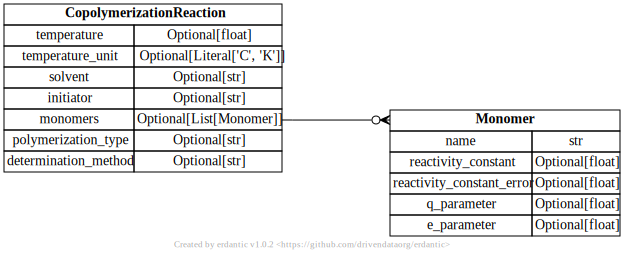
\includegraphics{constrained_decoding/index_files/figure-pdf/cell-4-output-1.svg}

}

\end{figure}

In this case, we will use PDF files in the form as images as input for
the model. To perform this conversion, we import some utilities.

\begin{Shaded}
\begin{Highlighting}[]
\ImportTok{from}\NormalTok{ pdf2image }\ImportTok{import}\NormalTok{ convert\_from\_path}
\ImportTok{from}\NormalTok{ utils }\ImportTok{import}\NormalTok{ process\_image, get\_prompt\_vision\_model}
\end{Highlighting}
\end{Shaded}

The code below only converts each page of the PDF into an image and then
generates dictionary objects in a format that can be used by the OpenAI
API.

\begin{Shaded}
\begin{Highlighting}[]
\NormalTok{filepath }\OperatorTok{=} \StringTok{\textquotesingle{}paper01.pdf\textquotesingle{}}
\NormalTok{pdf\_images }\OperatorTok{=}\NormalTok{ convert\_from\_path(filepath)}

\NormalTok{images\_base64 }\OperatorTok{=}\NormalTok{ [process\_image(image, }\DecValTok{2048}\NormalTok{, }\StringTok{\textquotesingle{}images\textquotesingle{}}\NormalTok{, filepath, j)[}\DecValTok{0}\NormalTok{] }\ControlFlowTok{for}\NormalTok{ j, image }\KeywordTok{in} \BuiltInTok{enumerate}\NormalTok{(pdf\_images)]}
\NormalTok{images }\OperatorTok{=}\NormalTok{ get\_prompt\_vision\_model(images\_base64}\OperatorTok{=}\NormalTok{images\_base64)}
\end{Highlighting}
\end{Shaded}

Armed with the images, we can now use the OpenAI API to extract the text
from the images. For this, we just call the API with our prompts and the
images.

\begin{Shaded}
\begin{Highlighting}[]
\NormalTok{completion }\OperatorTok{=}\NormalTok{ client.chat.completions.create(}
\NormalTok{    model}\OperatorTok{=}\StringTok{"gpt{-}4{-}turbo"}\NormalTok{,}
\NormalTok{    response\_model}\OperatorTok{=}\NormalTok{List[CopolymerizationReaction],}
\NormalTok{    max\_retries}\OperatorTok{=}\DecValTok{2}\NormalTok{,}
\NormalTok{    messages}\OperatorTok{=}\NormalTok{[}
\NormalTok{        \{}
            \StringTok{"role"}\NormalTok{: }\StringTok{"system"}\NormalTok{,}
            \StringTok{"content"}\NormalTok{: }\StringTok{"""You are a scientific assistant, extracting accurate information about co{-}polymerization reactions from scientific papers.}
\StringTok{Do not use data that was reproduced from other sources.}
\StringTok{If you confuse the reactivity ratios with other numbers, you will be penalized.}
\StringTok{Monomer names might be quite similar, if you confuse them, you will be penalized.}
\StringTok{NEVER combine data from different reactions, otherwise you will be penalized.}
\StringTok{If you are unsure, return no data. Quality is more important than quantity.}
\StringTok{"""}\NormalTok{,}
\NormalTok{        \},}
\NormalTok{        \{}
            \StringTok{"role"}\NormalTok{: }\StringTok{"user"}\NormalTok{,}
            \StringTok{"content"}\NormalTok{: }\StringTok{"""Extract the data from the paper into the provided data schema. We want an iterable of reaction objects and each reaction will be its own object. You can find each page of the paper as an image below.}
\StringTok{The relationship between monomers and parameters is typically indicated by subscripts that can be a number or an abbreviation of the monomer.}
\StringTok{Never return data that you are not absolutely sure about! You will be penalized for incorrect data."""}\NormalTok{,}
\NormalTok{        \},}
\NormalTok{        \{}\StringTok{"role"}\NormalTok{: }\StringTok{"user"}\NormalTok{, }\StringTok{"content"}\NormalTok{: [}\OperatorTok{*}\NormalTok{images]\},}
\NormalTok{    ],}
\NormalTok{    temperature}\OperatorTok{=}\DecValTok{0}\NormalTok{,}
\NormalTok{)}
\end{Highlighting}
\end{Shaded}

\begin{Shaded}
\begin{Highlighting}[]
\NormalTok{completion}
\end{Highlighting}
\end{Shaded}

\begin{verbatim}
[CopolymerizationReaction(temperature=60.0, temperature_unit='C', solvent='carbon tetrachloride', initiator='AIBN', monomers=[Monomer(name='methacrylic acid', reactivity_constant=0.54, reactivity_constant_error=0.01, q_parameter=None, e_parameter=None), Monomer(name='styrene', reactivity_constant=0.06, reactivity_constant_error=0.03, q_parameter=None, e_parameter=None)], polymerization_type='solution', determination_method='Kelen-Tudos'),
 CopolymerizationReaction(temperature=60.0, temperature_unit='C', solvent='chloroform', initiator='AIBN', monomers=[Monomer(name='methacrylic acid', reactivity_constant=0.51, reactivity_constant_error=0.01, q_parameter=None, e_parameter=None), Monomer(name='styrene', reactivity_constant=0.08, reactivity_constant_error=0.03, q_parameter=None, e_parameter=None)], polymerization_type='solution', determination_method='Kelen-Tudos'),
 CopolymerizationReaction(temperature=60.0, temperature_unit='C', solvent='acetone', initiator='AIBN', monomers=[Monomer(name='methacrylic acid', reactivity_constant=0.43, reactivity_constant_error=0.0, q_parameter=None, e_parameter=None), Monomer(name='styrene', reactivity_constant=0.65, reactivity_constant_error=0.02, q_parameter=None, e_parameter=None)], polymerization_type='solution', determination_method='Kelen-Tudos'),
 CopolymerizationReaction(temperature=60.0, temperature_unit='C', solvent='1,4-dioxane', initiator='AIBN', monomers=[Monomer(name='methacrylic acid', reactivity_constant=0.41, reactivity_constant_error=0.02, q_parameter=None, e_parameter=None), Monomer(name='styrene', reactivity_constant=0.59, reactivity_constant_error=0.05, q_parameter=None, e_parameter=None)], polymerization_type='solution', determination_method='Kelen-Tudos'),
 CopolymerizationReaction(temperature=60.0, temperature_unit='C', solvent='acetonitrile', initiator='AIBN', monomers=[Monomer(name='methacrylic acid', reactivity_constant=0.12, reactivity_constant_error=0.0, q_parameter=None, e_parameter=None), Monomer(name='styrene', reactivity_constant=0.29, reactivity_constant_error=0.0, q_parameter=None, e_parameter=None)], polymerization_type='solution', determination_method='Kelen-Tudos')]
\end{verbatim}

\bookmarksetup{startatroot}

\hypertarget{ocr-with-nougat}{%
\chapter{OCR with Nougat}\label{ocr-with-nougat}}

To run machine learning models on papers, we need to convert them into
plain text. This might require parsing PDFs, and sometimes optical
character recognition (OCR).

This is a difficult problem as not only the content of the paper needs
to be extracted, but also the layout can be important for the
interpretation of the paper. In addition, scientific papers often
contain mathematical formulas, which are not easy to parse.

To address those issues, researchers from Meta have trained the Nougat
system, which takes PDF as input and produces Markdown as output.

\hypertarget{cleaning-the-data}{%
\section{Cleaning the data}\label{cleaning-the-data}}

For certain applications it might be necessary to clean the data before
using it for other downstream tasks.



\end{document}
